\documentclass[border=3pt,tikz]{standalone}
% Gemeinsame Praeambel aller Abbildungen — Palette und Styles identisch zum
% GermEval-2026-Paper (Nuernberg NLP), damit die Bilder dort wiederverwendbar
% sind, ohne neu gezeichnet zu werden.
\usepackage{xcolor}
\usepackage{ifthen}
\usepackage{tikz}
\usetikzlibrary{shapes,arrows.meta,positioning,fit,backgrounds,calc,decorations.pathreplacing}

\definecolor{clrPrompt}{HTML}{B0CA97} % green  — Prompting (baseline)
\definecolor{clrSFT}{HTML}{E8A087}    % salmon — SFT (generative)
\definecolor{clrCls}{HTML}{88C4C8}    % teal   — ClsHead / FT (discriminative)
\definecolor{clrEns}{HTML}{D1BC8A}    % gold   — ensemble / majority vote
\definecolor{clrPCS}{HTML}{B7A0C9}    % purple — minority-class scope
\definecolor{clrBase}{HTML}{9AA0A6}   % grey   — untrained/frozen base

\tikzset{
  sysbox/.style={rectangle, rounded corners=3pt, line width=0.9pt,
    minimum width=2.7cm, minimum height=0.82cm, align=center,
    inner ysep=2pt, inner xsep=4pt, font=\fontsize{7.5}{9}\selectfont\bfseries},
  voterchip/.style={rectangle, rounded corners=1.5pt, line width=0.55pt,
    minimum width=0.78cm, minimum height=0.36cm, align=center,
    inner sep=1pt, font=\fontsize{5.4}{6.4}\selectfont},
  major/.style={rectangle, rounded corners=3pt, line width=0.9pt,
    align=center, font=\footnotesize\bfseries, inner ysep=4pt, inner xsep=10pt},
  io/.style={rectangle, rounded corners=2pt, line width=0.55pt, align=center,
    minimum width=1.35cm, minimum height=0.72cm, fill=black!3, draw=black!35,
    font=\fontsize{7.2}{8.6}\selectfont},
  bb/.style={rectangle, rounded corners=3pt, line width=0.8pt, align=center,
    minimum width=2.35cm, minimum height=0.86cm,
    font=\fontsize{7.4}{8.8}\selectfont},
  lab/.style={rectangle, rounded corners=1.2pt, line width=0.45pt,
    minimum height=0.30cm, align=center, inner sep=1.5pt,
    font=\fontsize{5.6}{6.8}\selectfont},
  edge/.style={-{Stealth[length=4pt]}, line width=0.6pt, black!50},
  bus/.style={line width=0.6pt, black!50},
  note/.style={font=\fontsize{6.4}{7.8}\selectfont\itshape, text=black!55,
    align=center},
  hdr/.style={font=\fontsize{6.5}{8}\selectfont\bfseries, text=black!55},
}

\begin{document}
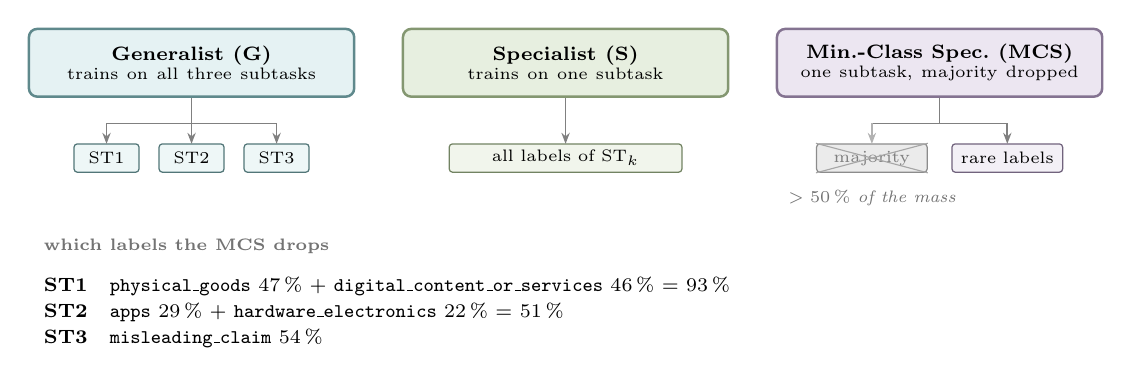
\begin{tikzpicture}[
  % Strenges Raster: drei gleich breite Spalten, eine Bus-Hoehe, eine
  % Chip-Hoehe. Jede Verbindung ist Bus + senkrechter Abgang — nie diagonal.
  scopebox/.style={sysbox, text width=3.85cm, minimum width=4.05cm,
    minimum height=0.86cm, font=\fontsize{6.9}{8.4}\selectfont\bfseries},
  chip/.style={lab, minimum height=0.36cm},
]

\def\ybox{1.55}   % Mitte der Scope-Box
\def\ybus{0.78}   % waagerechter Verteiler
\def\ychip{0.34}  % Mitte der Label-Chips

\def\cA{-4.75}
\def\cB{0}
\def\cC{4.75}

% ── Generalist ─────────────────────────────────────────────────────────────
\node[scopebox, draw=clrCls!70!black, fill=clrCls!22] (bA) at (\cA, \ybox)
  {Generalist (G)\\[-1.5pt]{\fontsize{5.8}{7}\selectfont\mdseries
   trains on all three subtasks}};
\draw[bus] (bA.south) -- (\cA, \ybus);
\draw[bus] ({\cA-1.08}, \ybus) -- ({\cA+1.08}, \ybus);
\foreach \dx/\lbl in {-1.08/ST1, 0/ST2, 1.08/ST3}{
  \node[chip, draw=clrCls!60!black, fill=clrCls!14, text width=0.72cm]
    (a\lbl) at ({\cA+\dx}, \ychip) {\lbl};
  \draw[edge] ({\cA+\dx}, \ybus) -- ({\cA+\dx}, {\ychip+0.18});
}

% ── Specialist ─────────────────────────────────────────────────────────────
\node[scopebox, draw=clrPrompt!75!black, fill=clrPrompt!30] (bB) at (\cB, \ybox)
  {Specialist (S)\\[-1.5pt]{\fontsize{5.8}{7}\selectfont\mdseries
   trains on one subtask}};
\draw[bus] (bB.south) -- (\cB, \ybus);
\node[chip, draw=clrPrompt!65!black, fill=clrPrompt!18, text width=2.85cm]
  (bl) at (\cB, \ychip) {all labels of ST$_k$};
\draw[edge] (\cB, \ybus) -- (\cB, {\ychip+0.18});

% ── Minority-class specialist ──────────────────────────────────────────────
\node[scopebox, draw=clrPCS!72!black, fill=clrPCS!26] (bC) at (\cC, \ybox)
  {Min.-Class Spec.\ (MCS)\\[-1.5pt]{\fontsize{5.8}{7}\selectfont\mdseries
   one subtask, majority dropped}};
\draw[bus] (bC.south) -- (\cC, \ybus);
\draw[bus] ({\cC-0.86}, \ybus) -- ({\cC+0.86}, \ybus);
\node[chip, draw=black!45, fill=black!8, text width=1.30cm] (mx)
  at ({\cC-0.86}, \ychip) {\textcolor{black!50}{majority}};
\draw[black!35, line width=0.4pt] (mx.south west) -- (mx.north east);
\draw[black!35, line width=0.4pt] (mx.north west) -- (mx.south east);
\node[chip, draw=clrPCS!62!black, fill=clrPCS!16, text width=1.30cm] (mk)
  at ({\cC+0.86}, \ychip) {rare labels};
\draw[edge, black!30] ({\cC-0.86}, \ybus) -- ({\cC-0.86}, {\ychip+0.18});
\draw[edge] ({\cC+0.86}, \ybus) -- ({\cC+0.86}, {\ychip+0.18});
\node[note, anchor=north] at ({\cC-0.86}, {\ychip-0.28}) {$>50\,\%$ of the mass};

% ── die Regel, kompakt ─────────────────────────────────────────────────────
\node[hdr, anchor=west] at (-6.75, -0.78)
  {\textsc{which labels the MCS drops}};
\node[anchor=north west, font=\fontsize{6.6}{9.4}\selectfont, text width=12.3cm]
  at (-6.75, -1.04)
  {\textbf{ST1}\quad \texttt{physical\_goods} 47\,\% $+$
   \texttt{digital\_content\_or\_services} 46\,\% $=$ 93\,\%\\
   \textbf{ST2}\quad \texttt{apps} 29\,\% $+$ \texttt{hardware\_electronics}
   22\,\% $=$ 51\,\%\\
   \textbf{ST3}\quad \texttt{misleading\_claim} 54\,\%};

\end{tikzpicture}
\end{document}
